\section{Physical Experiments}
\label{sec:physical-experiments}
Our previous experiments studied the effectiveness of Kit-Net for insertion tasks involving prismatic cavities. However, as shown in Fig.~\ref{fig:clamshell-objects} and Fig.~\ref{fig:clamshell-cavities}, many physical kitting tasks involve non-prismatic cavities. In this section, we study how Kit-Net can be used to kit objects in physical trials using depth images of the types of cavities shown in Fig.~\ref{fig:clamshell-cavities}. We call these \emph{conformal cavities}, as they ``conform" to some degree to the object shape. 

In these experiments we use a quaternion prediction network trained to predict the quaternion that will rotate a simulated depth image of an object to another simulated depth image of the same object in a different pose. We propose two possible methods for applying this trained network to kitting. Our first method is designed to work well with the clamshell cavities shown in Fig.~\ref{fig:clamshell-cavities}. Rather than image the hole of the cavity, we define a \emph{convex conformal cavity} to be the depth image of the inverted cavity. To obtain these depth images, we flip the cavity so the hole is pointing down and take a depth image of the positive mass of the cavity. The left image in Fig.~\ref{fig:clamshell-cavities} shows examples of these convex conformal cavities. Our second method works with a \emph{concave conformal cavity}, like that shown in Fig.~\ref{fig:mug-cavity-2} and the right image in Fig.~\ref{fig:clamshell-cavities}, that are formed as impressions into a surface. These types of cavities cannot simply be flipped upside down to obtain a depth image of their shape. Instead, we take a depth image of the actual cavity (where the cavity has negative mass) and rotate it 180\degree~about its principal axis.

We discuss the results for applying Kit-Net to novel convex conformal cavities in Section~\ref{subsubsec:real-positive} and to novel concave conformal cavities Section~\ref{subsubsec:real-negative}.
For the physical kitting experiments we measure success using a binary success metric for insertion by visually inspecting whether or not the object is completely contained in the target cavity.

\subsection{Physical Kitting into Convex Conformal Cavities}
\label{subsubsec:real-positive}

\begin{figure}[t]
  \vspace{8pt}
  \centering
  \begin{tikzpicture}[label/.style={inner sep=4pt, rounded corners=2pt, color=white, fill=black, fill opacity=0.25, text opacity=1, align=center, font=\footnotesize, yshift=2pt}]
    \node [inner sep=0] (img) {%
     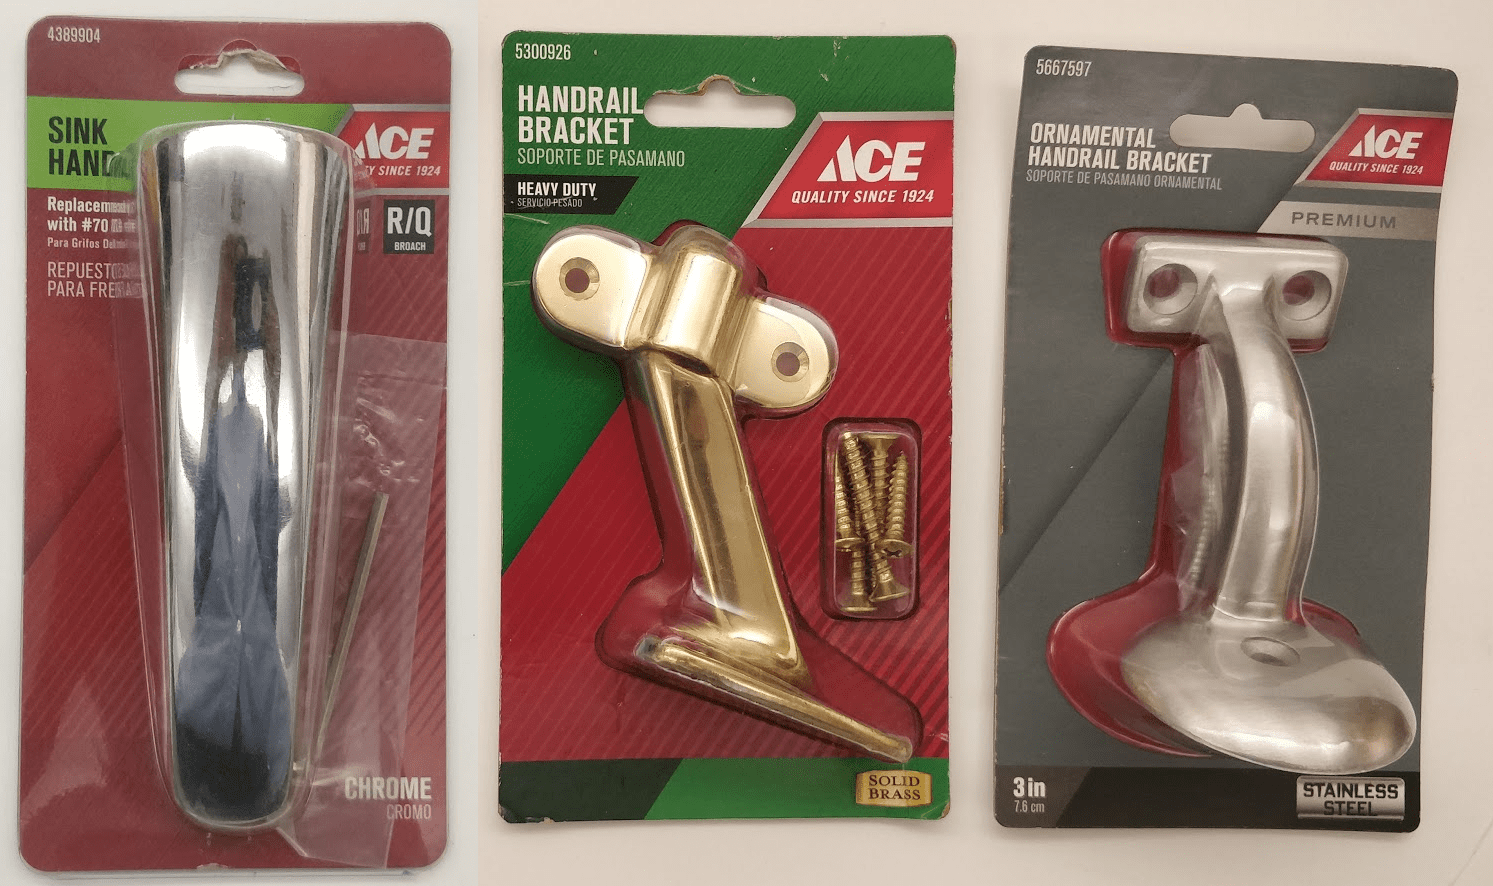
\includegraphics[width=\columnwidth]{figures/Three_Industrial_Objects.png}};
    \node [label, anchor=south west, xshift=14pt] at (img.south west) { Sink handle };
    \node [label, anchor=south, xshift=-4pt] at (img.south) { Handrail bracket };
    \node [label, anchor=south east, xshift=-14pt] at (img.south east) { Ornamental \\ handrail bracket };
  \end{tikzpicture}
  \caption{\textbf{Objects for Kit-Net Physical Experiments: }We use 3 packaged industrial objects that can be commonly found in a hardware store. 
   These objects were selected for their complex geometries, making precise orientation critical for effective kitting.}
  \label{fig:clamshell-objects}
\end{figure}

\begin{figure}[t]
  \centering
  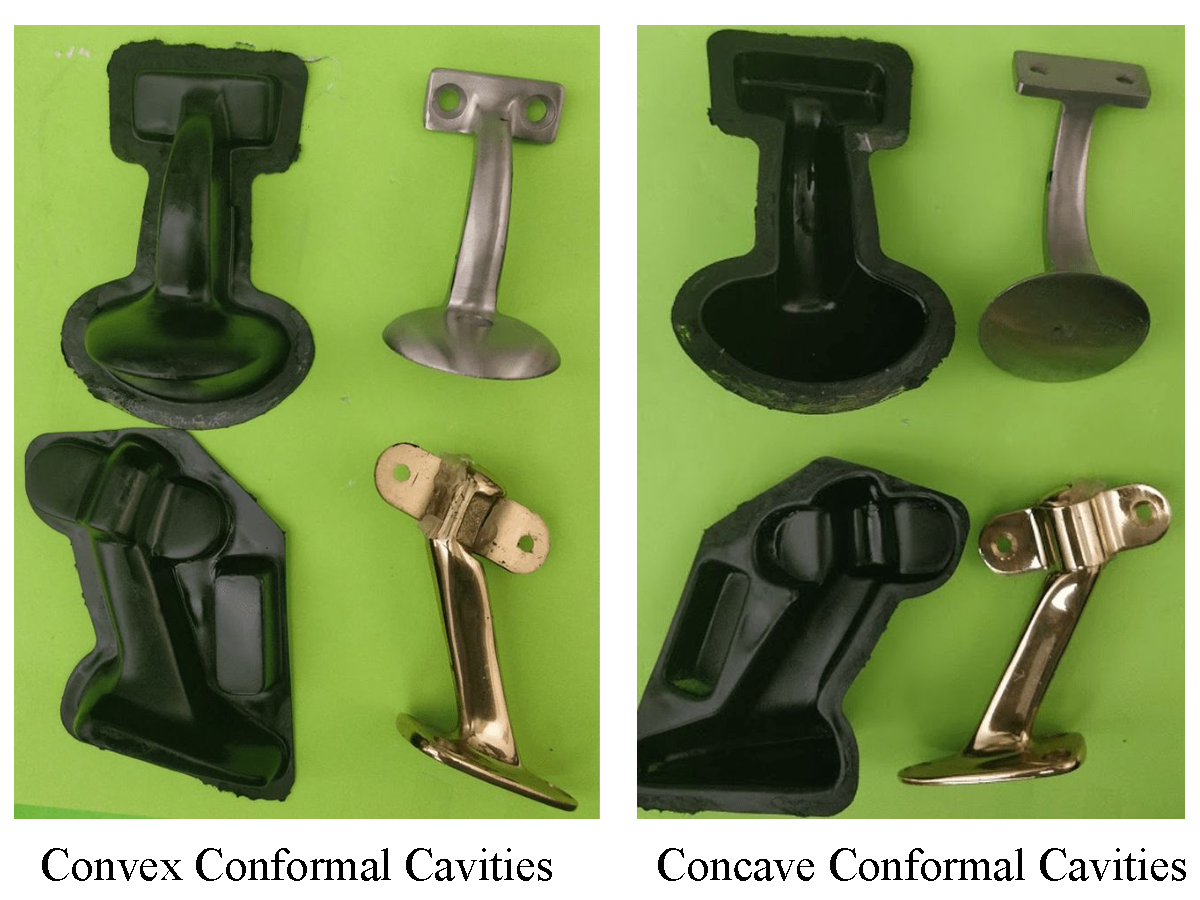
\includegraphics[width=\columnwidth]{figures/convex_concave_examples.pdf}
  \caption{\textbf{Examples of Physical Kitting Cavities: }The handrail bracket (bottom) and the ornamental handrail bracket (top), next to the corresponding convex cavity (left) and concave cavity (right).}
  \label{fig:clamshell-cavities}
\end{figure}

We also evaluate Kit-Net in physical kitting trials on an ABB-YuMi robot with a Photoneo depth camera, shown in Fig.~\ref{fig:splash}, using 4 packaged objects widely available in hardware stores and which are unseen during training (Fig.~\ref{fig:clamshell-objects}). %Figure~\ref{fig:toy-clamshells} visualizes packed toys widely available in retail stores. 
To prepare objects for kitting, we carefully extract each tool and kitting shell from its packaging and spray paint the shell to facilitate depth sensing as shown in Fig.~\ref{fig:clamshell-cavities}. We then place the kitting cavity open end down and image the cavity to generate $I^g$ before flipping it to expose its opening for the insertion task. For each trial, we insert the object into the cavity by hand, grasp it using the robot's suction gripper, translate it to be directly under the camera, and apply a random rotation of either $30\degree$ or $60\degree$, uniformly sampled from $SO(3)$ to simulate grasping the object from a bin in a non-uniform pose. Then, we flip the object such that the object faces the overhead depth camera and the suction cup grasp is occluded from the camera by the object. This process is illustrated in Fig.~\ref{fig:splash}. 

Kit-Net then orients the object using the learned controller, and matches centroids between the object and cavity for insertion before flipping it again and attempting to kit it. Table~\ref{table:positive-results} shows the number of successful kitting trials (out of 10 per object) of Kit-Net and the 2D baseline across 3 objects. We report a kitting trial as successful if the object is fully contained within the cavity from visual inspection. We observe that Kit-Net outperforms the baseline for 30\degree~initial rotations on 2 of the 3 objects, performing similarly to the baseline on the sink handle. We find that Kit-Net significantly outperforms the baseline on all objects for 60\degree~initial rotations.

Kit-Net's main failure modes are due to errors in the centroid matching procedure, as illustrated in Fig.~\ref{fig:failure-modes}. On the 30 degree sink handle task, Kit-Net aligned it correctly every time, but the centroid matching had it about ~0.5\,cm off, and there is no slack at the top of the cavity.


%\SJ{We can also add a table with success rate for each physical object that we tested on. Also comparison table with other methods using similar techniques example with- Zakka's method. In that case we can use similar items and also do a fit percentage comparison} 
% However, while \citet{zeng2020transporter} framed a 2D pick-and-place task given an image of an object and its place target by computing ${_s}T^g \in SE(2)$ through an efficient cross-convolution operation on GPU, we consider the best ${_s}T^g \in SE(2)$ by computing the best ${_s}R^g \in SO(2)$ that minimizes the chamfer distance between the point cloud representations of $I^s$ and $I^g$. 

\begin{table}[h]
\centering
\begin{tabular}{l c c c}\toprule 
 Object & Angle & 2D Baseline & Kit-Net \\
 \midrule
 Handrail bracket & 30\degree & 3/10 & \bf 10/10 \\ 
 Ornamental handrail bracket & 30\degree & 8/10 &  \bf 10/10 \\
 Sink handle & 30\degree & \bf 4/10 & 3/10 \\
 \addlinespace
 Handrail bracket & 60\degree & 1/10 & \bf 9/10 \\ 
 Ornamental handrail bracket & 60\degree & 2/10 & \bf 7/10 \\
 Sink handle & 60\degree & 0/10 & \bf 7/10 \\
 \bottomrule
\end{tabular}
\caption{\textbf{Physical Experiments Results for Convex Cavities: }We report the number of successful kitting trials for Kit-Net and the 2D baseline over 10 trials for 3 previously unseen objects with initial rotations of 30\degree and 60\degree. Results suggest that Kit-Net significantly outperforms the 2D baseline for initial rotations of 60\degree and outperforms the baseline for two out of three objects for initial rotations of 30\degree.}
\label{table:positive-results}
\end{table}
\subsection{Physical Kitting into Concave Conformal Cavities}
\label{subsubsec:real-negative}
%The positive cavity task provides a detailed depth image, but requires the cavity to first be presented at a flipped, 180\degree~rotation for imaging, which may not be feasible in an industrial environment. [this is a minor detail: omit. -KG 3/18]
Here, we perform the same experiment as in Section~\ref{subsubsec:real-positive}, but instead generate $I^g$ directly from an image of the cavity without flipping. Precisely, we segment out the cavity from an overhead depth image, deproject the depth image into its point cloud representation, and rotate the point cloud 180\degree~around its center of mass. Then, we project the rotated point cloud to the depth image $I^g$. %This process is illustrated in Fig.~\ref{fig:rotated-cavity}.

\begin{table}[h]
\centering
 \begin{tabular}{l c c c}\toprule
 Object & Angle & 2D Baseline & Kit-Net \\
 \midrule
 Handrail bracket & 30\degree & 0/10 & \bf 9/10 \\ 
 Ornamental handrail bracket & 30\degree & 0/10 & \bf 7/10 \\
 Sink handle & 30\degree & 1/10 & \bf 3/10 \\
 \addlinespace
 Handrail bracket & 60\degree & 0/10 & \bf 7/10 \\ 
 Ornamental handrail bracket & 60\degree & 0/10 & 0/10 \\
 Sink handle & 60\degree & 1/10 & \bf 4/10 \\
 \bottomrule
\end{tabular}
\caption{\textbf{Physical Experiments Results for Concave Cavities: }We report the number of successful kitting trials for Kit-Net and the 2D baseline over 10 trials for 3 previously unseen objects with initial rotations of 30\degree and 60\degree. Results suggest that Kit-Net significantly outperforms the baseline in all settings except for the handrail bracket with an initial rotation of 60\degree, for which neither Kit-Net nor the baseline can successfully kit the object.}
\label{table:negative-results}
\end{table}

Table~\ref{table:negative-results} shows results from experiments with 3 novel objects from Fig.~\ref{fig:clamshell-objects} across 10 controller rollouts. We observe that Kit-Net outperforms the baseline for initial rotations of both 30 and 60 degrees on the handrail bracket and sink handle, and for an initial rotation of 30 \degree for the ornamental handrail bracket. For the ornamental handrail bracket, the depth image from the concave cavity is low quality as shown in Fig.~\ref{fig:failure-modes} (center image), causing Kit-Net to fail when the object is 60 degrees away the correct insertion orientation. We examined this failure and found that it occurs because the cavity for the neck of the bracket is very thin, making it difficult to obtain a good depth image. Kit-Net also has low performance on the sink handle due to small errors in centroid matching, as discussed in the prior section. Fig.~\ref{fig:failure-modes} (bottom left) shows an example failure case where the sink handle is correctly oriented but the translation is slightly off. There were also occasional cases (Fig.~\ref{fig:failure-modes} (top left)) where the suction gripper occludes the handle of the ornamental handrail bracket. In these cases, the robot can only see the base, resulting in failure.

% \begin{figure}
  \centering
  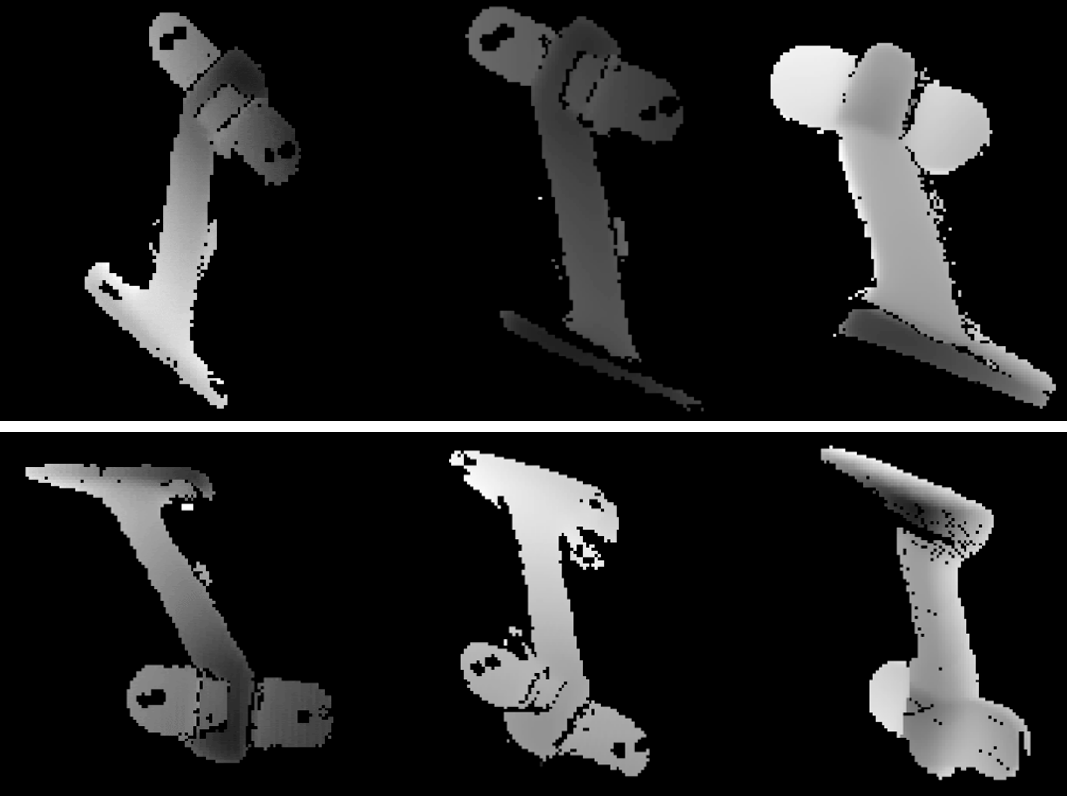
\includegraphics[width=0.48\textwidth]{figures/Orientation.PNG}
  \caption{\AB{this figure needs some labels, eg. $I^s$, $\hat{I}^g$, $I^g$}\textbf{Reorienting Objects with Kit-Net: }Kit-Net aligns objects from $I^s$ (left) to $\hat{I}^g$ (middle) given both positive (top right) and negative (bottom right) goal images $I^g$ by estimating ${_s}\hat{t}^g \in SE(3)$. Positive goal images are generated as described in Section~\ref{subsubsec:real-positive} while negative goal images are generated as described in Section~\ref{subsubsec:real-negative}.}
  \label{fig:Kit-Net-to-cavity}
\end{figure} OMIT -KG 3/18

\begin{figure}[t]
  \vspace{8pt}
  \centering
  % "Break between images" -KG
%   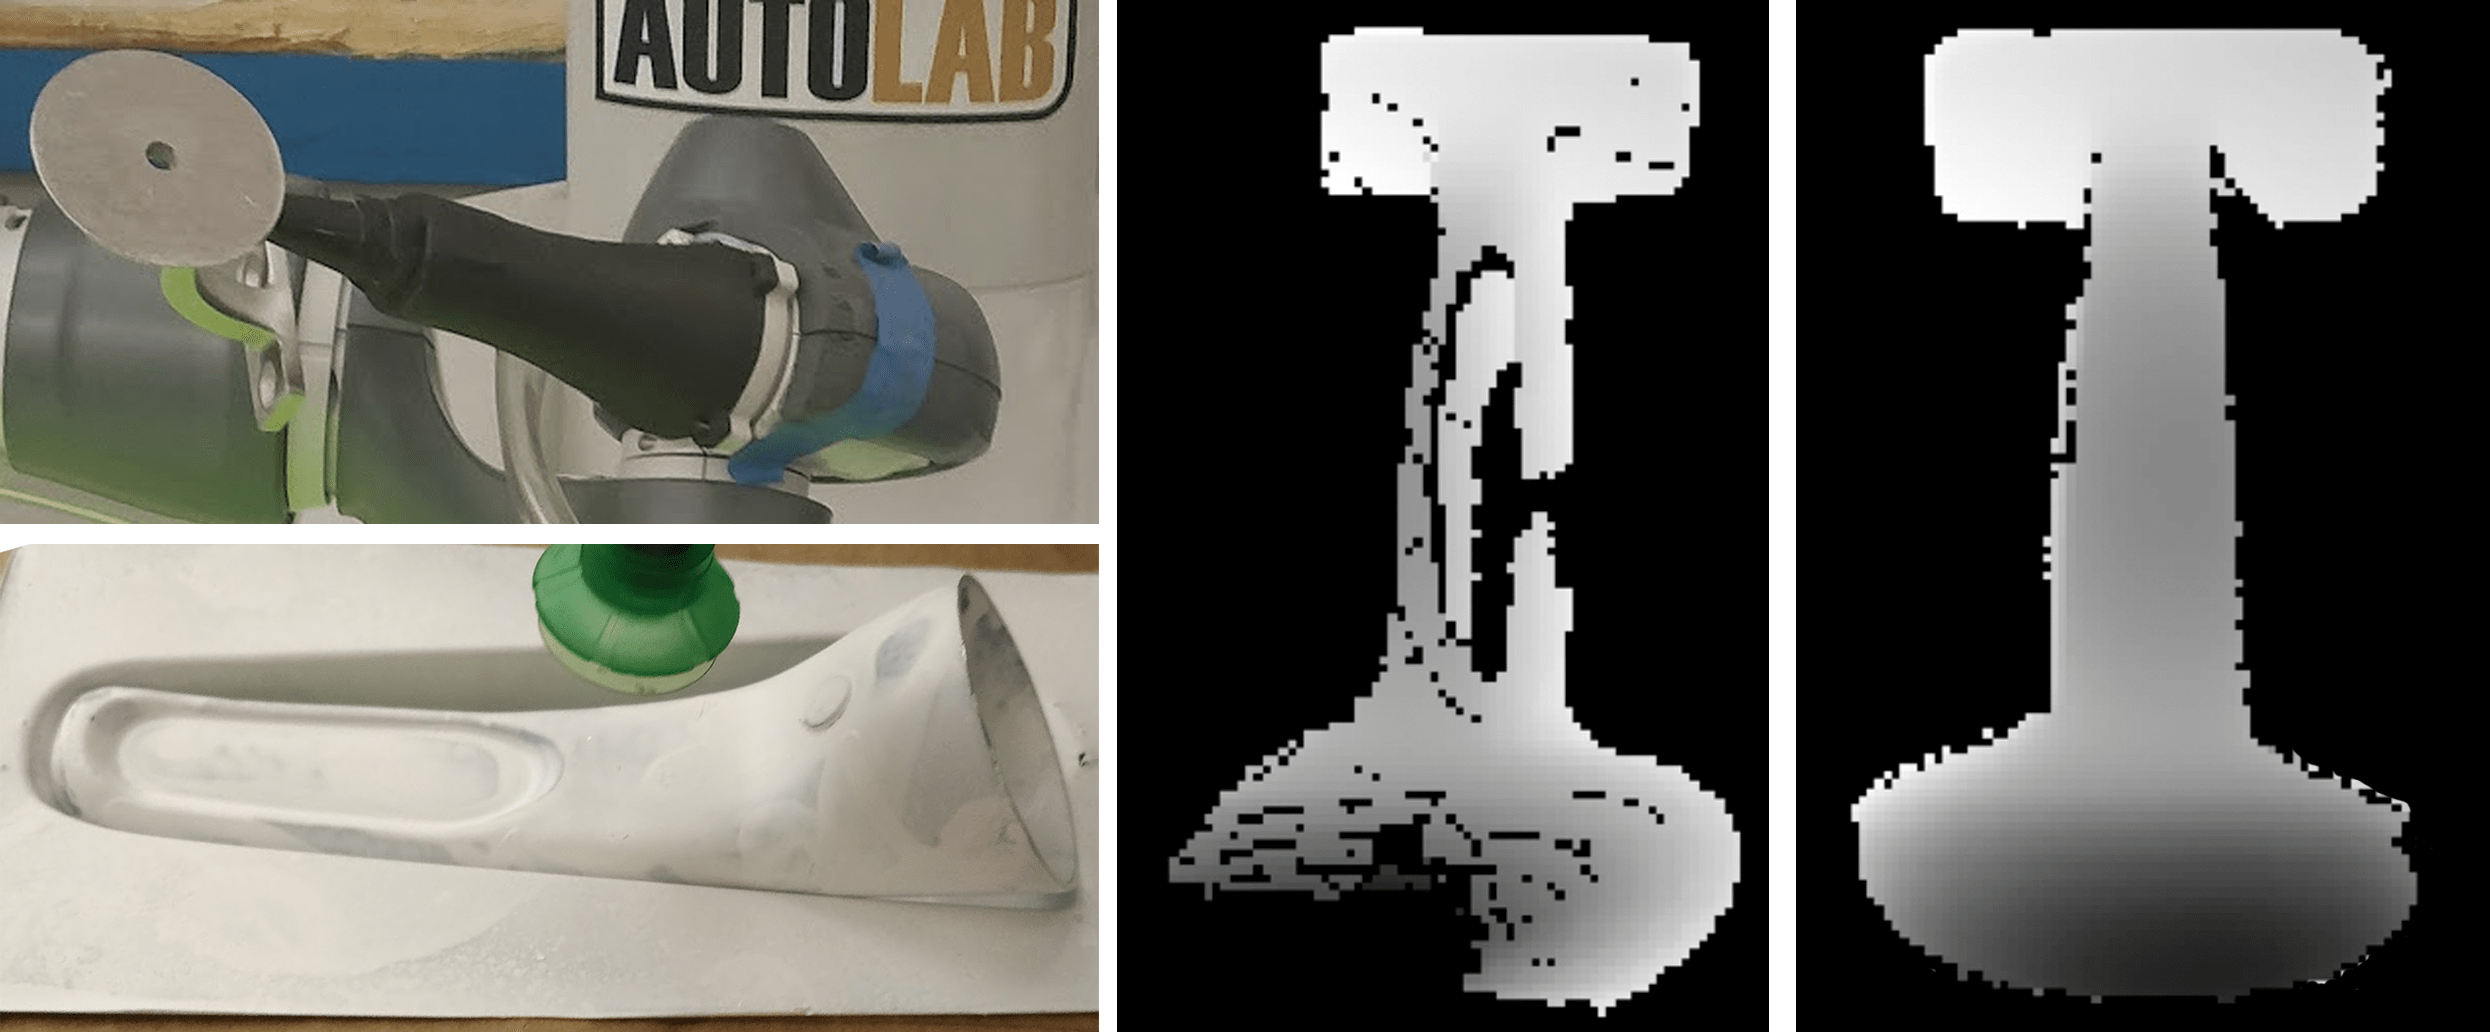
\includegraphics[width=0.48\textwidth, trim=0 488 0 0, clip]{figures/Failure Cases.png} \\[2pt]
%   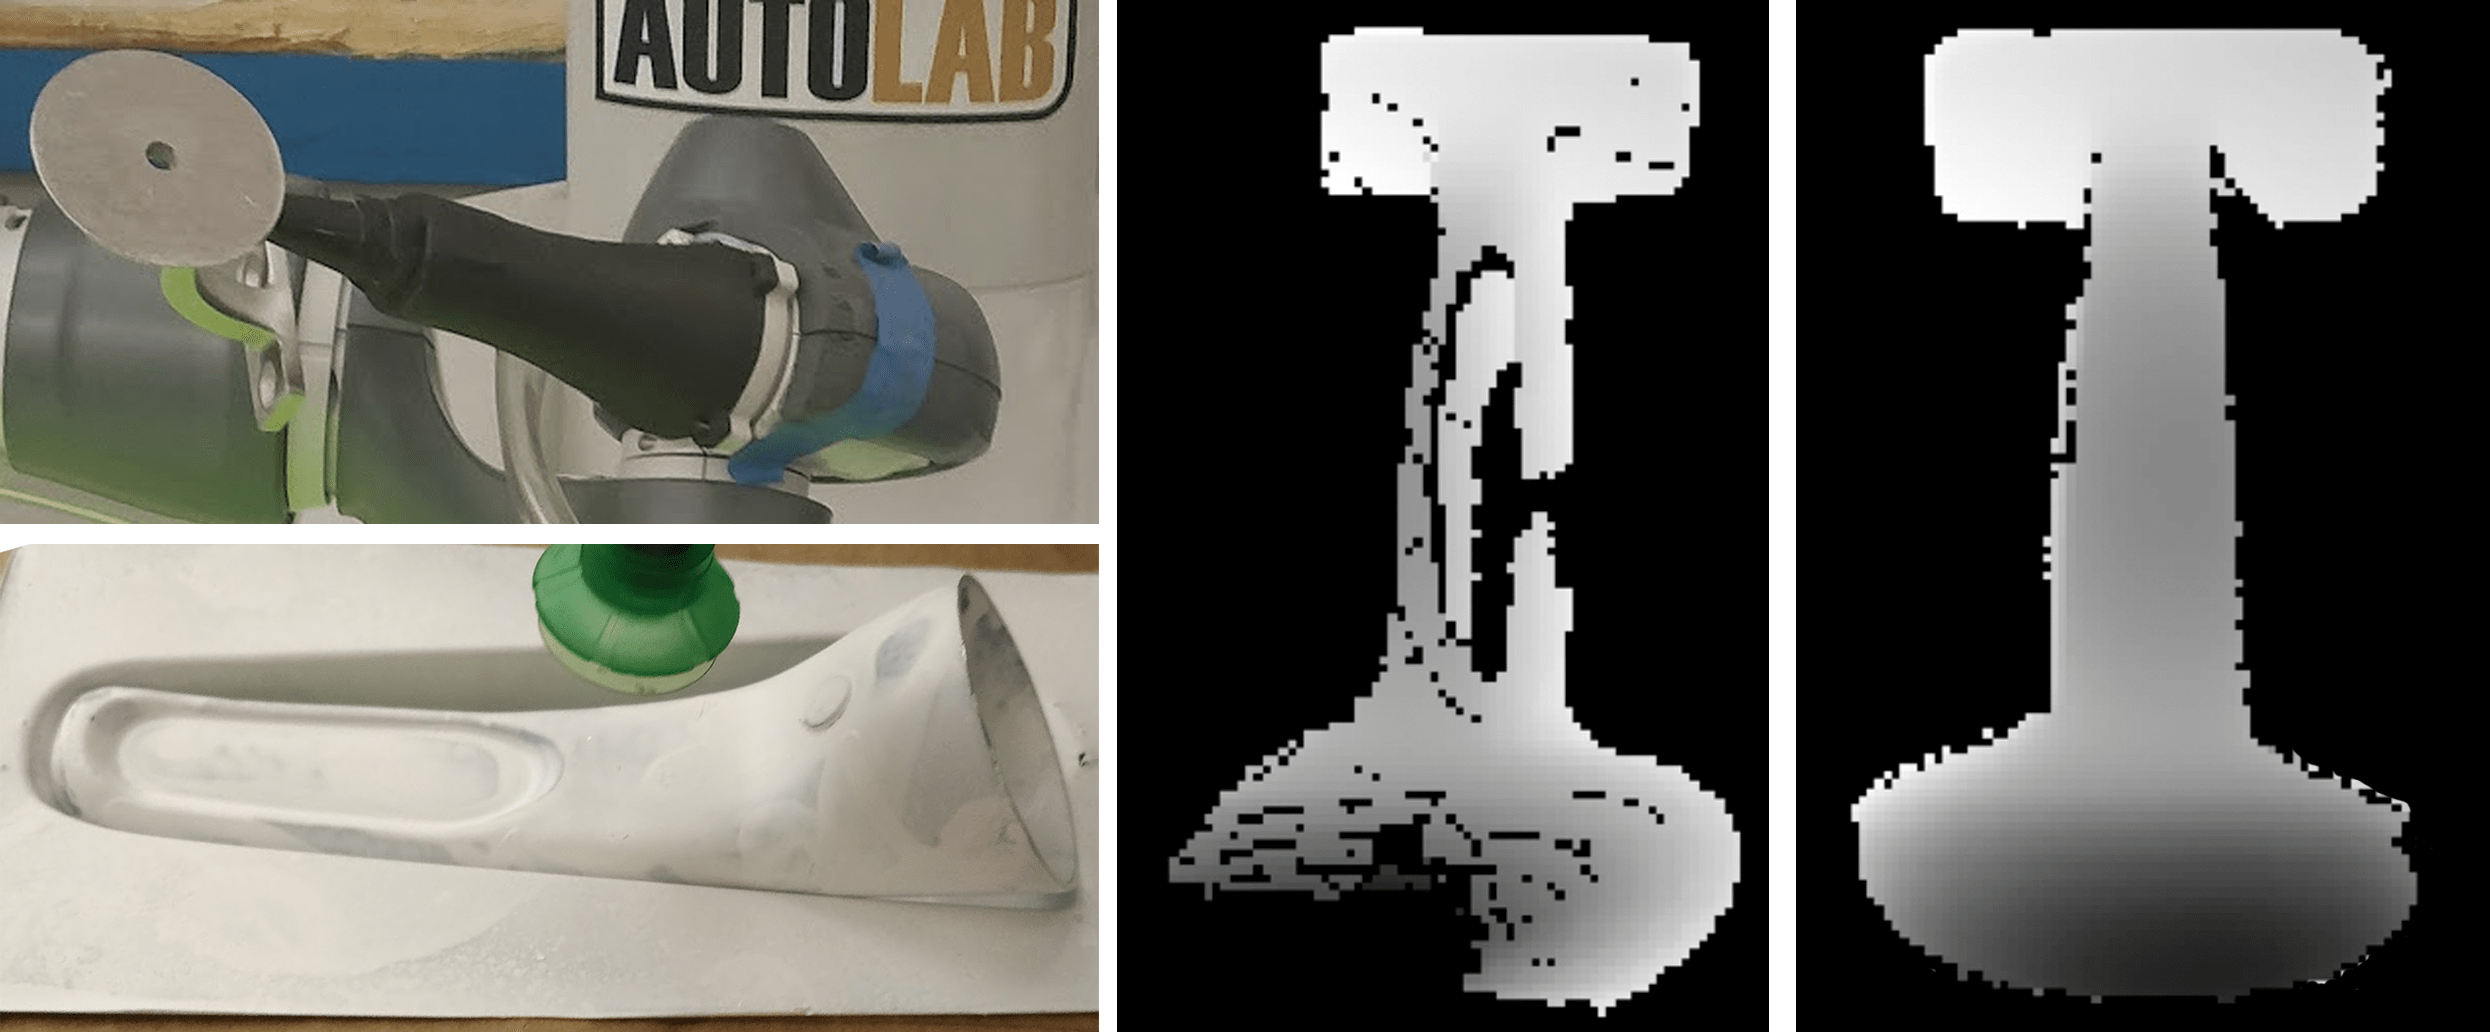
\includegraphics[width=0.48\textwidth, trim=0 0 0 636, clip]{figures/Failure Cases.png}
  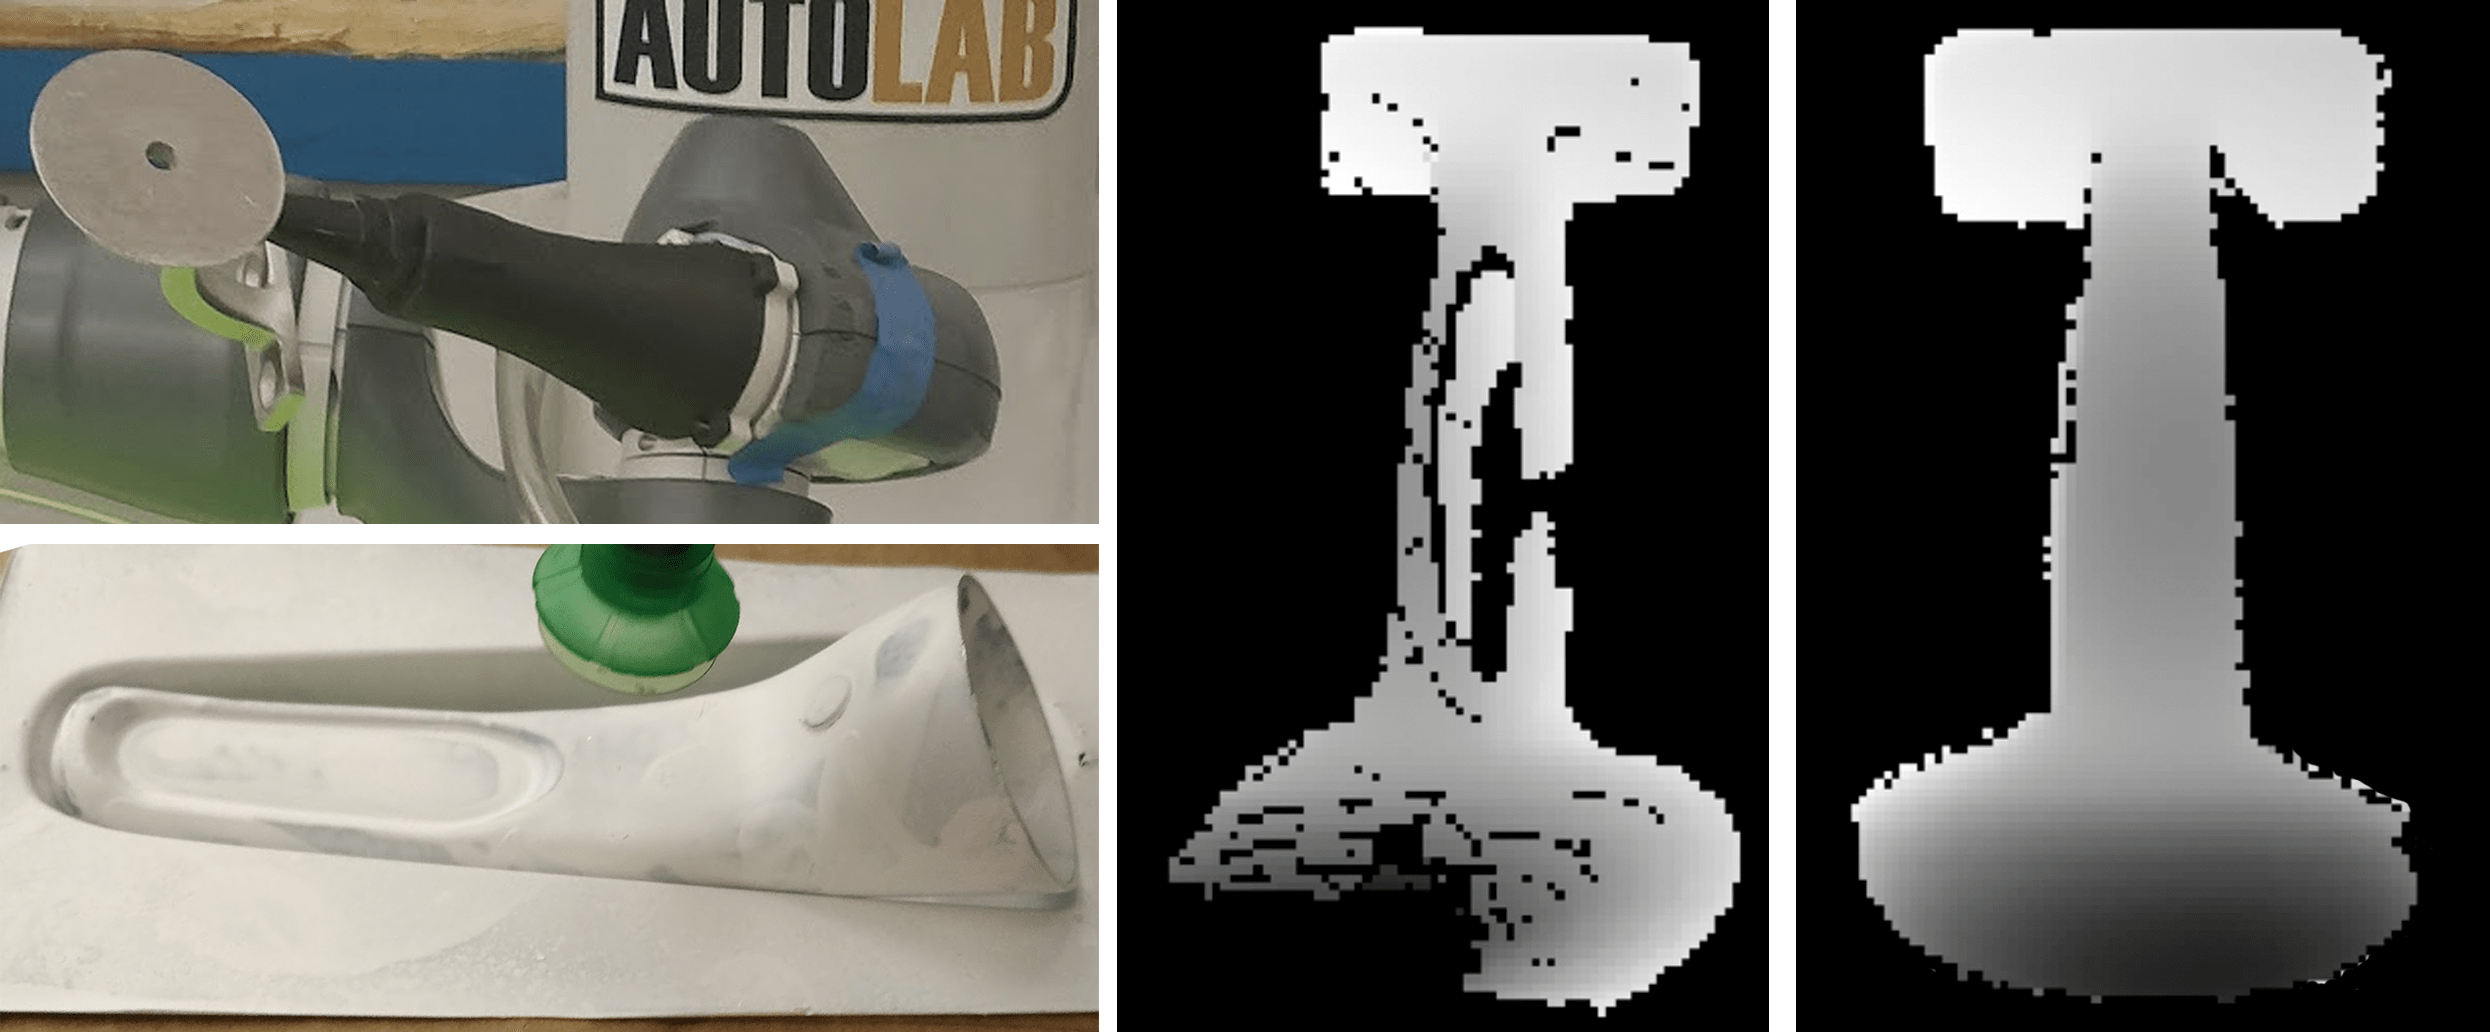
\includegraphics[width=0.48\textwidth]{figures/Failure Cases.png}
  \caption{\textbf{Kit-Net Failure Cases: } The top-left image shows a configuration of the ornamental handrail bracket
  %that results in self-occlusion; the downward-facing depth camera cannot image
  where the suction gripper occludes
  the handle below the base. The bottom-left image shows the sink handle. Although Kit-Net was able to orient the handle correctly for insertion, the centroid matching had a small error in estimating translation and the cavity does not have enough slack to be properly inserted. The center and right images show depth images for the ornamental handrail bracket for the concave conformal cavity and convex conformal cavity, respectively.
  %using the process described in \ref{subsec:real-negative}, and the right image shows the depth image of the cavity positive as described in \ref{subsec:real-positive}.
  The inside of the concave cavity is very thin and the angle of the camera makes it hard to perfectly image it, resulting in a poor depth image (center image). % using the method of \ref{subsec:real-negative}.
  This leads to 0 successes for both the baseline and for Kit-Net when the initial rotation is 60\degree{} away from the desired rotation for kitting.}
  \label{fig:failure-modes}
\end{figure}


% \begin{figure}
  \centering
  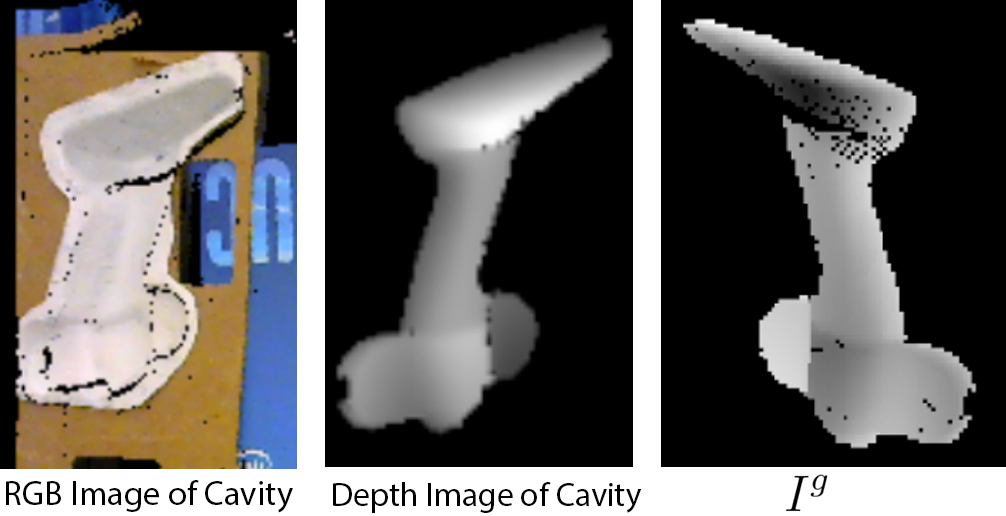
\includegraphics[width=0.48\textwidth]{figures/Rotated_Negative.png}
  \caption{\textbf{Generating Negative Goal Images: }After taking the original image (left), we segment out all parts that don't belong to the cavity (middle). Then, we project from depth to point cloud, rotate the pointcloud about its centroid, and deproject to depth image to get $I^g$ (right).}
  \label{fig:rotated-cavity}
\end{figure}
 OMIT -KG 3/18
